\documentclass{sig-alternate-05-2015}

\usepackage{multirow}
\usepackage{color}
\usepackage{algorithm}
\usepackage{algorithmic}
\usepackage{mathrsfs}
\DeclareMathOperator*{\argmin}{argmin}
\DeclareMathOperator*{\argmax}{argmax}

%\newcommand{\cheng}[1]{\textcolor{green}{\textbf{Cheng: }{\footnotesize #1}}}
%\newcommand{\lexing}[1]{\textcolor{red}{\textbf{Lexing: }{\footnotesize #1}}}
%\newcommand{\dawei}[1]{\textcolor{blue}{\textbf{Dawei: }{\footnotesize #1}}}

\newcommand{\etal}{{\em et al.}\xspace}
\usepackage{url}
\usepackage{hyperref}
\newcommand{\surl}[1]
{
	\urlstyle{same}\url{#1}
}

\usepackage[svgnames]{xcolor}
\definecolor{navy}{rgb}{0.1, 0.1, 0.8}
\definecolor{gray}{rgb}{0.4, 0.4, 0.4}

\newcommand{\eat}[1]{}
\newcommand{\rev}[1]{{\color{navy}{#1}}}
\newcommand{\verify}[1]{{\color{red}{#1}}}
\usepackage{soul} %% needed for highlighting
\newcommand{\TODO}[2]{ { [{\bf #1}:~{\hl{#2}}]}}

% place holder spacing hacks
%\newcommand{\secmoveup}{\vspace{-0.0mm}}                %{\vspace{-0.12in}}
\newcommand{\secmoveup}{\vspace{-0.12mm}}                %{\vspace{-0.12in}}
\newcommand{\bigsecmoveup}{\secmoveup\vspace{-.0mm}}   %{\vspace{-0.08in}}
\newcommand{\textmoveup}{\vspace{-0.mm}}               %{\vspace{-0.08in}}
\newcommand{\bigtextmoveup}{\textmoveup\vspace{-0.0in}} %{\vspace{-0.06in}}
\newcommand{\itemmoveup}{\vspace{-0mm}}              %{\vspace{-0.04in}}
%\newcommand{\eqmoveup}{\vspace{-0.0in}}                 %{\vspace{-0.16in}}
\newcommand{\eqmoveup}{\vspace{-0.04in}}                 %{\vspace{-0.16in}}
%\newcommand{\captionmoveup}{\eqmoveup\vspace{-0.0in}}   %{\vspace{-0.16in}}
\newcommand{\captionmoveup}{\eqmoveup\vspace{-0.16in}}   %{\vspace{-0.16in}}
\newcommand{\refitemmoveup}{\vspace{-0mm}}            %{\vspace{-0.16in}}

\begin{document}


\CopyrightYear{2016}
\setcopyright{acmcopyright}
\conferenceinfo{CIKM'16 ,}{October 24-28, 2016, Indianapolis, IN, USA}
\isbn{978-1-4503-4073-1/16/10}\acmPrice{\$15.00}
\doi{http://dx.doi.org/10.1145/2983323.2983672}

\clubpenalty=10000
\widowpenalty = 10000
% using \vfill\eject just before the bib items in .bbl file will force the bib items below to the next page or column to help rectify the bad break

\title{Learning Points and Routes to Recommend Trajectories}

\numberofauthors{3}
\author{
    \alignauthor Dawei Chen$^{*\dagger}$\\
    \alignauthor Cheng Soon Ong$^{*\dagger}$\\
    \alignauthor Lexing Xie$^{*\dagger}$\\
    \and
    $^*$The Australian National University, $^\dagger$Data 61, CSIRO, Australia\\
    \and
    \{u5708856, chengsoon.ong, lexing.xie\}@anu.edu.au
}

% The code below should be generated by the tool at
% http://dl.acm.org/ccs.cfm
% Please copy and paste the code instead of the example below.
\begin{CCSXML}
<ccs2012>
<concept>
<concept_id>10002951.10003317.10003338.10003343</concept_id>
<concept_desc>Information systems~Learning to rank</concept_desc>
<concept_significance>500</concept_significance>
</concept>
<concept>
<concept_id>10002951.10003317.10003347.10003350</concept_id>
<concept_desc>Information systems~Recommender systems</concept_desc>
<concept_significance>500</concept_significance>
</concept>
<concept>
<concept_id>10003120.10003130.10003233.10010519</concept_id>
<concept_desc>Human-centered computing~Social networking sites</concept_desc>
<concept_significance>300</concept_significance>
</concept>
</ccs2012>
\end{CCSXML}

\ccsdesc[500]{Information systems~Learning to rank}
\ccsdesc[500]{Information systems~Recommender systems}
\ccsdesc[300]{Human-centered computing~Social networking sites}

\maketitle

\begin{abstract}
%!TEX root = main.tex

The problem of recommending tours to travellers is an important and broadly studied area.
Suggested solutions include various approaches of points-of-interest (POI)
recommendation and route planning.
We consider the task of recommending a sequence of POIs 
%as a tour to travellers
, that simultaneously uses information about POIs and routes.
Our approach unifies the treatment of various sources of information
by representing them as features in machine learning algorithms, enabling us to
learn from past behaviour. %without specialised treatment of spatial, temporal or social information.
Information about POIs are used to learn a POI ranking model
that accounts for the start and end points of tours.
Data about previous trajectories are used for learning transition patterns between POIs that
enable us to recommend probable routes.
In addition, a probabilistic model is proposed
%and a Structured Support Vector Machine are used
to combine the results of POI ranking and the POI to POI transitions.
We propose a new F$_1$ score on pairs of POIs
that capture the order of visits.
Empirical results show that our approach improves on
recent methods, and demonstrate that
combining points and routes enables better trajectory recommendations.

\end{abstract}

%\printccsdesc  % print CCS
\keywords{Trajectory recommendation; Learning to rank; Planning}

%!TEX root = main.tex

\section{Introduction}
\label{sec:intro}

\begin{figure}[ht]
	\centering
	%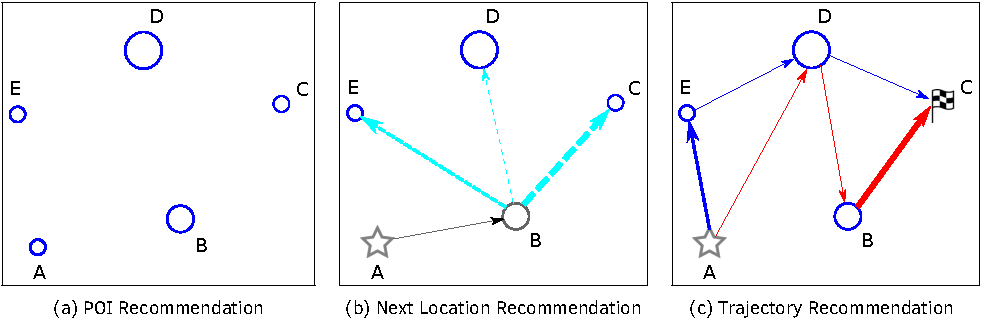
\includegraphics[width=0.7\textwidth]{fig/fig1-flavours.pdf}
	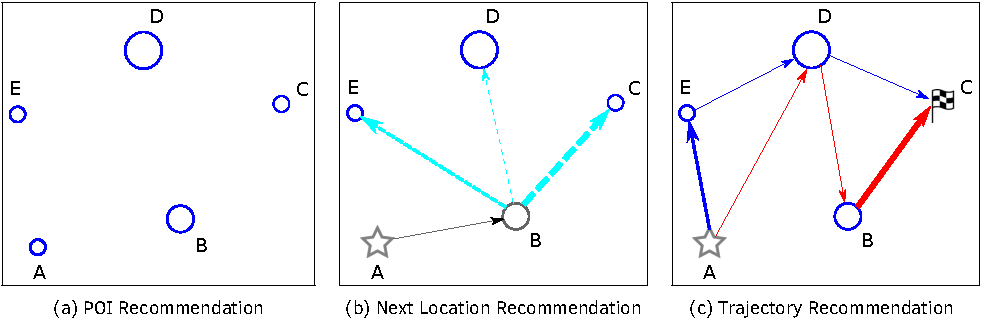
\includegraphics[width=\columnwidth]{fig/fig1-flavours.pdf}
	\caption{Three settings of trajectory recommendation problems. 
Node size: POI score; edge width: transition score between pairs of POIs; 
%grey: input query; 
grey: observed;
star: starting location; flag: ending location. See Section~\ref{sec:intro} for details.
}
	\label{fig:threesettings}
\end{figure}



This paper proposes a novel solution to recommend travel routes in cities.
A large amount of location traces are becoming available from ubiquitous location tracking devices.
For example, FourSquare
%, the local search and discovery service, 
has 50 million monthly users who have made 8 billion check-ins~\cite{4sq},
and Flickr
%, the online photo-sharing site, 
hosts over 2 billion geo-tagged public photos~\cite{flickr}. 
Such large amounts of travel data provide new opportunities for better
travel planning traditionally done with written travel guides.
%for example, choosing and ranking locations for a variety of activities from dining to recreation,
%and potential new solutions to orienteering and routing problems.
Good solutions to these problems will in turn lead to better urban experiences for residents and visitors alike, and foster sharing of even more location-based behavioural data.

%!TEX root = main.tex

%\section{Related Work}
%\label{sec:relatedwork}

There are several settings of recommendation problems for locations and routes, as illustrated in Figure~\ref{fig:threesettings}.
We summarise recent work most related to formulating and solving learning problems on assembling routes from POIs,
and refer the reader to a number of recent surveys~\cite{bao2015recommendations,zheng2015trajectory,zheng2014urban} for general overviews of the area.
%There are three settings of recommendation problems for locations and routes, as illustrated in Figure~\ref{fig:threesettings}.
The first setting can be called POI recommendation (Figure~\ref{fig:threesettings}(a)). Each location (A to E) is scored with geographic and behavioural information such as category, reviews, popularity, spatial information such as distance, and temporal information such as travel time uncertainty, time of the day or day of the week.
This can be in discovery mode, such as identifying points-of-interest~\cite{zheng2009mining,li2015instagram} and includes efficient querying of geographic objects for trips ~\cite{hashem2015efficient}.
A popular approach is based on the collaborative filtering model
for learning user-location affinity~\cite{shi2011personalized}, with additional ways to incorporate spatial~\cite{lian2014geomf,liu2014exploiting}, temporal~\cite{yuan2013timeaware,hsieh2014mining,gao2013temporal}, or spatial-temporal~\cite{yuan2014graph} information.

Figure~\ref{fig:threesettings}(b) illustrates the second setting: next location recommendation.
Here the input is a partial trajectory (e.g. started at point A and currently at point B), the task of the algorithm is to score the next candidate location (e.g, C, D and E) based on the perceived POI score and transition compatibility with input $A\rightarrow B$.
It is a variant of POI recommendation except given both the user and locations travelled to date. The solutions to this problem include incorporating Markov chains into collaborative filtering~\cite{fpmc10,ijcai13,zhang2015location},
quantifying tourist traffic flow between points-of-interest~\cite{zheng2012patterns},
formulating a binary decision or ranking problem~\cite{baraglia2013learnext}, and with sequence models such as recurrent neural networks~\cite{aaai16}.


This paper considers the final setting: trajectory recommendation (Figure~\ref{fig:threesettings}(c)). Here the input are some factors about the desired route, e.g. starting point A and end point C, along with auxiliary information such as the desired length of trip. The algorithm needs to take into account location desirability (as indicated by node size) and transition compatibility (as indicated by edge width), and compare route hypotheses such as A-D-B-C and A-E-D-C. Existing work in this area either uses heuristic combination of locations and routes~\cite{lu2010photo2trip,ijcai15,lu2012personalized}, or formulates an optimisation problem that is not informed or evaluated by behaviour history~\cite{gioniswsdm14,chen2015tripplanner}.
%Joint learning of location preferences and routes remains an open problem.
%Our work is in this category. We formulate a learning problem to score the whole trajectory, taking into account individual POI properties and relationships among different POIs.
%
We note, however, that two desired qualities are still
missing from the current solutions to trajectory recommendation.
The first is principled method to jointly learn POI ranking (a prediction problem)
and optimise for route creation (a planning problem).
The second is a unified way to incorporate various features
such as location, time, distance, user profile and social interactions,
as they tend to get specialised and separate treatments.
This work aims to address these challenges. %bridge these gaps.
We propose a novel way to learn point and route preferences jointly.
In Section~\ref{sec:feature}, we describe the features that are used to ranking points,
and POI-POI transitions that are factorised along %five
different types of location properties.
Section~\ref{sec:recommendation} details a number of our proposed approaches to recommend trajectories.
%leveraging techniques including learning to rank, Markov chain inference and route planning.
%%
%%
\eat{
Our solution consists of several parts.
We propose a learning to rank formulation to capture the preference of POIs given the starting and ending points of a trajectory (Section~\ref{sec:method}).
We model pair-wise transition patterns between POIs by factorising the transition likelihoods along five different types of location properties,
which alleviates data sparsity between each pair of POIs and allows POIs of the same type and neighbourhood to share parameters.
We combine the results of point and transition ranking using Markov chain inference and route planning techniques (Section~\ref{sec:recommendation}).
We further propose a novel way to jointly learn point and transition scores with a Structured Support Vector Machine (StructuredSVM).
In Section~\ref{sec:experiment},
}
%%
%%
We evaluate the proposed algorithms on trajectories from five different cities in Section~\ref{sec:experiment}.
% with a traditional metric F$_1$ on POIs as well as a novel pairs-F$_1$ metric specifically designed for trajectories (Section~\ref{sec:experiment}).
The main contributions of this work are:
%\begin{itemize}
%\setlength{\itemsep}{-2pt}
%\item We propose a novel algorithm to jointly optimise point preference and route plan.
%Our approach is feature-driven and learns from past behaviour without having to design specialised treatment for spatial, temporal or social information.
%\item We show good performance compared to recent results~\cite{ijcai15}, and also quantify the contributions from different components,
%such as ranking points, scoring transitions, and routing.
%\item We propose a new metric to evaluate trajectories: pairs-F$_1$,
%which takes into account both the point identity and the visiting orders in a trajectory.
%Our benchmark data and results are publicly available.
%\end{itemize}
\begin{itemize}
\setlength{\itemsep}{-2pt}
\item We propose a novel algorithm to jointly optimise point preferences and routes. We find that learning-based approaches generally outperform heuristic route recommendation~\cite{ijcai15}.
Incorporating transitions to POI ranking results in a better sequence of POIs, and avoiding sub-tours further improves performance of classical Markov chain methods.
\item Our approach is feature-driven and learns from past behaviour without having to design specialised treatment for spatial, temporal or social information. It incorporates information about location, POI categories and behaviour history, and can use additional time, user, or social information if available.
\item We show good performance compared to recent results~\cite{ijcai15}, and also quantify the contributions from different components, such as ranking points, scoring transitions, and routing.
\item We propose a new metric, pairs-F$_1$, to evaluate trajectories.
%which takes into account both the point identity and the visiting orders in a trajectory.
It captures the order in which POIs are visited. 
pairs-F$_1$ lies between 0 and 1, and achieves 1 if and only if the recommended trajectory is exactly the same as the ground truth. Our benchmark data and results are at \surl{https://bitbucket.org/d-chen/tour-cikm16}.
\end{itemize}

\section{POI, Query and Transition}
\label{sec:feature}
\secmoveup


We aim to recommend a particular tour such that the user will visit a sequence of POIs, denoted $p_1, \ldots, p_L$, that maximises utility. We are given the desired start ($p_1=p_s$) and end point ($p_L=p_e$), and an associated number $L$ of POIs desired, from which we propose a trajectory through the city.
%
%In Figure~\ref{fig:threesettings}(c), an example tour is shown in blue, which starts at the POI denoted as a grey star, visits two intermediate POIs, and terminates on the fourth POI denoted as a flag. The tour of length 4 can be modelled as a sequence of directed edges in a graph containing POIs in the city as nodes.
%
The training data consists of a set of tours of varying length in a particular city. We assume that all POIs %$\mathcal{P}$ 
in the city are visited at least once by some user, and hence can construct a graph with POIs as nodes and potentially multiple directed edges between each pair of nodes. 
%The set of categories are shown in Figure~\ref{fig:poicats} in the appendix, and the popularity is defined as the number of distinct users that visited the POI\cite{ht10}.



%\subsection{POI Features and Query}
%\label{sec:poifeature}

We extract the category, popularity (number of distinct visitors)~\cite{ht10}, total number of visits and average visit duration for each POI.
%A naive approach would be to recommend the trajectory based on the popularity (number of distinct visitors)~\cite{ht10} of POIs only,
%that is we always suggest the top-$k$ most popular POIs for all visitors given the start and end location, 
%and its only adaptation to a particular request is to adjust $k$ to match the desired length.
%In addition to popularity, 
%we can also rank the candidate POIs based on the other three POI specific features (category, total visits and average duration).
Furthermore, since we are constrained by the fact that trajectories have to be of length $L$ and start and end at certain points, we hope to improve the recommendation by using this information.
In other words, using the \textit{query} $q = (p_s, p_e, L)$ we can construct new features by contrasting candidate POIs with $p_s$ and $p_e$.
%
For each of the POI features (category, popularity, total visits and average duration),
we construct two new features by taking the difference of the feature in POI $p$ with $(p_s, p_e)$ respectively.
For the category, we set the feature to $1$ when their categories are the same and $-1$ otherwise.
For popularity, total visits and visit duration, we take the real valued difference.
Lastly, we compute the distance from POI $p$ to $p_s$ (and $p_e$) using the Haversine formula~\cite{haversine},
and also include the required length $L$ of the trajectory as a feature.



%\subsection{Transition probabilities}
%\label{sec:transition}


\begin{figure}[t]
%\includegraphics[width=\textwidth]{fig/poi_transmat.png}
\includegraphics[width=\columnwidth]{fig/poi_transmat.png}
\caption{Example of transition matrices for two POI features: POI categories and neighborhood
These statistics are from the Melbourne dataset. See Section~\ref{sec:feature} for descriptions.}
\label{fig:transmat}\captionmoveup
\end{figure}


In addition to information about each individual POI, a tour recommendation system would benefit
from capturing the likelihood of transitioning between different POIs. One option would be to
directly model the probability of going from one POI to another, but this has several weaknesses:
Such a model would be unable to handle a new POI (one that has not yet been visited).
Furthermore, even if we restrict ourselves to known POIs, there may be many locations which
are rarely visited, leading to significant challenges in estimating the probabilities from
empirical data.

We model POI transitions using a Markov chain with discrete %factored
states by factorising the transition probability of ($p_i$ to $p_j$) %from POI $p_i$ to POI $p_j$ 
as a product of transition probabilities between pairs of individual POI features, %(listed in Section~\ref{sec:poifeature}),
assuming independence between these features.
POIs are grouped into $5$ clusters using K-means according to their geographical locations to reflect their neighbourhood relations.
%We directly model the transition between the category and neighbourhood of each POI as the conditional probability.
The popularity, total number of visits and average visit duration are discretised by binning
them uniformly into $5$ discrete intervals on the log scale.
%Transition matrices of individual POI features are computed using maximum likelihood estimation.
The POI-POI transition matrix can be efficiently computed by taking the Kronecker product of
the transition matrices for the individual features, which are estimated using maximum likelihood principle, 
then updating it based on two additional constraints (and appropriately normalised).
First we disallow self-loops by setting the probability of ($p_i$ to $p_i$) to zero.
Secondly, when a group of POIs have identical (discretised) features, we distribute the probability uniformly among POIs in the group. 
Figure~\ref{fig:transmat} visualises the transition matrices for two of the POI features in Melbourne.
%More details of this procedure are provided in the Appendix.

\section{Tour Recommendation}
\label{sec:recommendation}

%In this section, we describe a number of approaches to recommend trajectories that leverage POI ranking and/or route planning.

\subsection{POI Ranking and Route Planning}
\label{sec:rankplan}

A naive approach would be to recommend the trajectory based on the popularity (number of distinct visitors)~\cite{ht10} of POIs only,
that is we always suggest the top-$k$ most popular POIs for all visitors given the start and end location.
We call this baseline approach \textsc{PoiPopularity},
and its only adaptation to a particular request is to adjust $k$ to match the desired length.

On the other hand, we can leverage the whole set of POI features described in Section~\ref{sec:feature}
to learn a ranking of POIs using rankSVM with linear kernel and $L2$ loss~\cite{lranksvm},
\begin{equation*}
\min_{\mathbf{w_r}} \frac{1}{2} 
                     \|\mathbf{w_r}\|^2 + 
%                    \mathbf{w_r}^T \mathbf{w_r} + 
%                    C_r \sum_{(p_i, q_n), (p_j, q_n) \in \mathcal{P} \times \mathcal{Q}}
%                    C_r \sum_{p_i, p_j \in \mathcal{P}, q_n \in \mathcal{Q}}
                    \underset{p_i, p_j \in \mathcal{P}, q_n \in \mathcal{Q}}{C_r ~\sum}
                    \max \left( 0,~ 1 - \mathbf{w_r}^T (\phi_{i,n} - \phi_{j,n}) \right)^2,
\end{equation*}
where $\mathbf{w_r}$ is the parameter vector,
$C_r > 0$ is a regularisation constant.
$\mathcal{P}$ is the set of POIs to rank,
$\mathcal{Q}$ is the queries corresponding to trajectories in training set,
and $\phi_{i,n}$ is the feature vector for POI $p_i$ with respect to the query $q_n \in \mathcal{Q}$.

For training the rankSVM, the labels are generated using the number of occurrences of
POI $p$ in trajectories grouped by query $(p_s, p_e, L)$,
without counting the occurrence of $p$ when it is the origin or destination of a trajectory.
We create an algorithm, \textsc{PoiRank}, to recommend trajectory by first ranking POIs 
%utilising both POI and query specific features described above. 
%\textsc{PoiRank} 
then takes the top ranked $L-2$ POIs and connects them in sequence according to the ranks.



%\subsection{Route Planning}
%\label{sec:markov}

In addition to recommend trajectory by ranking POIs, we can leverage the POI-POI transition probabilities and 
recommend a trajectory with respect to a query by maximising the (log) likelihood. 
The maximum likelihood solution can be found using a variant of the Viterbi algorithm (with emission probabilities ignored).
We call this approach that only uses the transition probabilities between POIs as \textsc{Markov}.

%which is shown in Algorithm~\ref{alg:markov}.
%The entry $A[l, p]$ in score matrix $A$ stores the maximum likelihood associated with the (partial) trajectory 
%that starts from $p_s$ and ends at $p$ with $l$ POI visits, 
%and entry $B[l, p]$ in the backtracking-point matrix $B$ stores the predecessor of $p$ in that (partial) trajectory.



\subsection{Combine Ranking and Transition}
\label{sec:rank+markov}


\eat{
Recall that in Section~\ref{sec:ranksvm} we described how to recommend trajectories by ranking points,
i.e., \textsc{PoiRank} % and its simplified variant \textsc{PoiPopularity}.
While algorithms based on points ranking utilise POI and/or query features, 
the transitions between POIs are never considered.
and ones that consider transitions between POIs, i.e., \textsc{Markov} and \textsc{MarkovPath}.
only use POI-POI transitions but ignoring the point ranks.
In this section, we propose three approaches to %now in a position to 
jointly optimise the recommendation with both POI preferences and route plans.
We want to leverage both POI ranking and POI-POI transitions when recommending trajectories.
A summary of the various trajectory recommendation approaches can be found in Table~\ref{tab:algsummary}.
}


%\subsection{POI ranking and transitions}
%\label{sec:rank+markov}

Instead of recommend trajectory by either ranking POIs or planning routes with regard to POI-POI transition probabilities, 
%To recommend the \textit{most likely} trajectory with respect to a query,
%we want to combine the ranking of POIs with the transition probabilities,
we would like to leverage both point ranking and transitions,
i.e., recommending a trajectory that maximise the points ranking of its POIs as well as its likelihood at the same time.
To begin with, we transform the ranking scores of POIs with respect to query $q$
to a probability distribution using the softmax function,
%~\cite{bishop2006},
\vspace{-0.5em}
\begin{equation*}
\label{eq:rankprob}
P_R(p_j | q) = \frac{\exp(R_j)}{\sum_j \exp(R_j)},
\end{equation*}
where $R_j$ is the ranking score of POI $p_j$ from rankSVM with respect to query $q$.

%  \item Heuristics: \textsc{Rank+Markov}, \textsc{Rank+MarkovPath}
One heuristic to find a trajectory that simultaneously maximise the ranking probabilities of its POIs and its likelihood 
could be optimising the following objective:
\begin{equation*}
    \argmax_{\mathcal{T} \in \mathcal{P}^L} ~\alpha \sum_{k=1}^{L} \log P_R(p_{j_k} | q) +
                                     (1-\alpha) \sum_{k=1}^{L-1} \log P(p_{j_{k+1}} | p_{j_k}),
\end{equation*}
such that
$p_{j_1} = p_s, ~ p_{j_L} = p_e$ and
$p_{j_k} \in \mathcal{P}, ~1 \le k \le L$.
$\mathcal{T} = (p_{j_1}, \dots, p_{j_L})$ is any possible trajectory,
$\alpha \in [0, 1]$ is a parameter to trade-off the importance between the point ranking and transition, 
%of POIs and the POI-POI transitions in the recommended trajectory, 
and can be tuned using cross validation in practice.
%Similar to the \textsc{Markov} algorithm mentioned above, 
Let $S(p; p', q)$ be a convex combination of point ranking and transition,
\begin{equation*}
    S(p; p', q)  = \alpha \log P_R(p|q) + (1-\alpha) \log P(p|p') \},
\end{equation*}
then the best path (or walk) can be found using the Viterbi algorithm with the two recursions below,
%with both node and transition scores. 
%The objective can be optimised by adapting the Viterbi algorithm and using the two recursions below,
%A[l+1, p] = \max_{p' \in \mathcal{P}} \{ A[l, p'] + \alpha \log P_R(p|q) \\ + (1-\alpha) \log P(p|p') \}
%B[l+1, p] = \argmax_{p' \in \mathcal{P}} \{ A[l, p'] + \alpha \log P_R(p|q) \\ + (1-\alpha) \log P(p|p') \}
\begin{alignat}{2}
&A[l+1, p]   &&= \max_{p' \in \mathcal{P}} \{ A[l, p'] + S(p; p', q) \}, \label{eq:max} \\
&B[l+1, p]   &&= \argmax_{p' \in \mathcal{P}} \{ A[l, p'] + S(p; p', q) \}, \label{eq:argmax}
\end{alignat}
where $A$ is the score matrix, and entry $A[l, p]$ stores the maximum value associated with the (partial) trajectory
that starts at $p_s$ and ends at $p$ with $l$ POI visits.
$B$ is the backtracking-point matrix, and entry $B[l, p]$ stores the predecessor of $p$ in that (partial) trajectory.

The maximum objective value is $A[L, p_e]$,
and the corresponding trajectory can be found by tracing back from $B[L, p_e]$.
We call this approach that uses both the points ranking and transitions \textsc{Rank+Markov},
with pseudo code shown in Algorithm~\ref{alg:rank+markov}.


\begin{algorithm}[t]
\caption{\textsc{Rank+Markov}: recommend trajectory with POI ranking and transition}
\label{alg:rank+markov}
\begin{algorithmic}[1]
\STATE \textbf{Input}: $\mathcal{P}, p_s, p_e, L$
\STATE \textbf{Output}: Trajectory $\mathcal{T} = (p_s, \cdots, p_e)$ with $L$ POIs
%\STATE Compute a rank $<_{p_i, p_j} \subset \mathcal{P}^2$ w.r.t. query $q = (p_s, p_e, L)$
%\STATE Compute POI-POI transition matrix
\STATE Initialise score matrix $A$ and backtracking pointers $B$
\FOR{$p \in \mathcal{P}$}
    \STATE $A[2, p] = \alpha \log P_R(p_s|q) + S(p; p_s, q)$
    \STATE $B[2, p] = p_s$
\ENDFOR
\FOR{$l=2$ to $L-1$}
    \FOR{$p \in \mathcal{P}$}
        \STATE Compute $A[l+1, p]$ using Equation~(\ref{eq:max})
        \STATE Compute $B[l+1, p]$ using Equation~(\ref{eq:argmax})
    \ENDFOR
\ENDFOR
% //trace back to find the actual path
\STATE $\mathcal{T}= \{p_e\}$, $l = L$, $p = \mathcal{T}.first$
\REPEAT
    \STATE Prepend $B[l, p]$ to $\mathcal{T}$
    \STATE $l = l - 1$, $p = \mathcal{T}.first$
\UNTIL{$l < 2$}
\RETURN $\mathcal{T}$
\end{algorithmic}
\end{algorithm}






\subsection{Avoiding sub-tours} %%LX: walk vs path is never defined! but sub-tour seem to be??
\label{sec:nosubtour}

Trajectories recommended by \textsc{Markov} (Section~\ref{sec:rankplan}) and \textsc{Rank+Markov} (Section~\ref{sec:rank+markov})
are found using the maximum likelihood approach, and may contain multiple visits to the same POI.
This is because the best solution from Viterbi decoding %best path (or walk) from Viterbi decoding %random walk suggested by Viterbi 
may have 
%tottering (where the Markov chain transitions back and forth between two states), or may have 
circular sub-tours (where a POI already visited earlier in the tour is visited again).
We propose a method for eliminating sub-tours by %specifying additional constraints. % when recommending trajectories.
%
%  \item ILP
%In particular, we find the best path using an integer linear program (ILP) with
finding the best path using an integer linear program (ILP) with
sub-tour elimination constraints adapted from the Travelling Salesman Problem~\cite{opt98}.
In particular, given a set of POIs $\mathcal{P}$, the POI-POI transition matrix and a query $q = (p_s, p_e, L)$,
we recommend a trajectory by solving the following ILP:
\begin{alignat}{5}
& \max  ~&& \sum_{i=1}^{N-1} \sum_{j=2}^N x_{ij} \log P(p_j | p_i)                                                 \nonumber \\
& ~s.t. ~&& x_{ij} \in \{0, 1\}, ~x_{ii} = 0, ~u_i \in \mathbf{Z}, ~\forall i, j = 1, \cdots, N                    \label{eq:cons1} \\
&        && \sum_{j=2}^N x_{1j} = \sum_{i=1}^{M-1} x_{iN} = 1, ~\sum_{i=2}^N x_{i1} = \sum_{j=1}^{N-1} x_{Nj} = 0  \label{eq:cons2} \\
&        && \sum_{i=1}^{N-1} x_{ik} = \sum_{j=2}^N x_{kj} \le 1,   ~\forall k=2, \cdots, N-1                       \label{eq:cons3} \\
&        && \sum_{i=1}^{N-1} \sum_{j=2}^N x_{ij} = L-1,                                                            \label{eq:cons4} \\
&        && u_i - u_j + 1 \le (N-1) (1-x_{ij}),                     \forall i, j = 2, \cdots, N                    \label{eq:cons5}
\end{alignat}
where $N=|\mathcal{P}|$ is the number of available POIs and $x_{ij}$ is a binary decision variable 
that determines whether transition from $p_i$ to $p_j$ would be allowed in the recommended trajectory.
For brevity, we arrange the POIs such that $p_1 = p_s$ and $p_N = p_e$.
%assume $x_{i1}$ and $x_{1j}$ represent the incoming and outgoing transitions of $p_s$,
%similarly, $x_{iN}$ and $x_{Nj}$ correspond to the incoming and outgoing transitions of $p_e$.
%Constraint $(\ref{eq:cons2})$ restricts that %only one outgoing (incoming) transition for $p_s$ ($p_e$) is permitted, i.e., 
%Constraint $(\ref{eq:cons3})$ restricts that any POI could be visited at most once.
%Constraint $(\ref{eq:cons4})$ restricts that only $L-1$ transitions between POIs are permitted, 
Firstly, the recommended trajectory should start from $p_s$ and end at $p_e$ (Constraint~\ref{eq:cons2}),
in addition, any POI could be visited at most once (Constraint~\ref{eq:cons3}).
Moreover, only $L-1$ transitions between POIs are permitted (Constraint~\ref{eq:cons4}),
i.e., the number of visited POIs should be exactly $L$ (including $p_s$ and $p_e$).
The last constraint, where $u_i$ is an auxiliary variable, 
enforces that only a single sequence of POIs without sub-tours is permitted in the recommended trajectory.
We call our method that uses the transition matrix to recommend paths 
%that do not have circular sub-tours \textsc{MarkovPath}.
without circular sub-tours \textsc{MarkovPath}.


%Similar to the \textsc{Markov} algorithm (Section~\ref{sec:rankplan}),
Sub-tours in trajectories recommended by \textsc{Rank+Markov} can be eliminated in a similar manner,
we solve an ILP by optimising Objective~(\ref{eq:obj2}) with the same constraints described above.
This algorithm is called \textsc{Rank+MarkovPath} in the experiments.
%simply replace Objective~(\ref{eq:obj}) with \ref{eq:obj2}.
\vspace{-1.5em}
\begin{equation}
\label{eq:obj2}
\max \sum_{i=1}^{N-1} \sum_{j=2}^N ~x_{ij} ~S(p_j; p_i, q).
\end{equation}

%sub-tours may appear in trajectories recommended by \textsc{Rank+Markov} algorithm (Section~\ref{sec:rank+markov}).
%we can optimise Objective~(\ref{eq:rank+markovpath}) using ILP with the same constraints described above.
%we solve an ILP with Objective~(\ref{eq:rank+markovpath})
%We eliminate sub-tours by solving an ILP to maximise objective 
%$\sum_{i=1}^{N-1} \sum_{j=2}^N x_{ij} S(p_j; p_i, q)$ 
%with respect to constraints (\ref{eq:cons1}) to (\ref{eq:cons5}) described above.
%\begin{equation}
%\label{eq:rank+markovpath}
%\max \sum_{i=1}^{N-1} \sum_{j=2}^N x_{ij} (\alpha \log P_R(p_j | q) + (1-\alpha) \log P(p_j | p_i))
%\max \sum_{i=1}^{N-1} \sum_{j=2}^N ~x_{ij} ~S(p_j; p_i, q).
%\end{equation}



\eat{
\subsection{Structured SVM}
\label{sec:ssvm}
\secmoveup

As trajectory is a sequence of POI visits,
%given query $q = (p_s, p_e, L)$, we can model the desired trajectory $\mathcal{T}$
it is natural to model the desired trajectory %$\mathcal{T}$ with respect to query $q = (p_s, p_e, L)$
as a chain of discrete variables, where each variable has $|\mathcal{P}|$ states.
Structured prediction can incorporates both the features of variables (unary features) and
the features of interactions between neighbouring variables (pairwise features) to make a
prediction,
\begin{displaymath}
    \mathcal{T}^* = \argmax_{\mathcal{T} \in \mathcal{P}^L} 
                    \sum_{j=1}^L \mathbf{w_u}^T \mathbf{\phi}_j + \sum_{j=1}^{L-1} \mathbf{w_p}^T \mathbf{\phi}_{j, j+1}
\end{displaymath}
where $L$ is the number of expected POI visits, 
$\mathbf{\phi}_j$ are features of the $j$-th variable,
$\mathbf{\phi}_{j, j+1}$ are the pairwise features between the $j$-th and $(j+1)$-th variables, 
$\mathbf{w_u}$ and $\mathbf{w_p}$ are the parameters of unary and pairwise features respectively.

We construct the unary features from the POI ranking and pairwise features from POI-POI transitions.
In particular, unary features are defined as ranking probabilities (Equation~\ref{eq:rankprob}),
recall that we have a query consisting of start ($p_s$) and end ($p_e$) locations, 
which we model as a $1$-of-$K$ encoding in the unary features.
Pairwise features are defined from the transition probabilities %$P(p_j | p_i)$ 
described in Section~\ref{sec:feature}.
%
% describe SSVM training (1-slack formulation)
To estimate the parameters, we train a Structured Support Vector Machine using the 1-slack formulation~\cite{ssvm09},
\begin{align*}
    \min_{\mathbf{w}} & ~\frac{1}{2} \|\mathbf{w}\|^2 + C \xi \\
    s.t. & ~\forall \left( \bar{\mathcal{T}}_1, \cdots, \bar{\mathcal{T}}_M \right) \in \mathscr{T}^M: \\
         & \frac{1}{M} \mathbf{w}^T \sum_{i=1}^M \left[ \Psi(q_i, \mathcal{T}_i) - \Psi(q_i, \bar{\mathcal{T}}_i) \right] \ge 
           \frac{1}{M} \sum_{i=1}^M \Delta(\mathcal{T}_i, \bar{\mathcal{T}}_i) - \xi,
\end{align*}
where $\mathbf{w} = [\mathbf{w_u}^T, \mathbf{w_p}^T]^T$ is the parameter vector,
$C$ is a regularisation constant, $\xi \ge 0$ is the slack variable, $M$ is the training set size, 
$q_i$ is the query corresponds to the $i$-th trajectory in training set.
$\mathcal{T}_i$ and $\bar{\mathcal{T}}_i$ are the $i$-th trajectory and its corresponding prediction respectively.
$\Psi$ is a joint feature map~\cite{joachims2009predicting} built from the unary and pairwise features with regard to
 a query and a label (the ground truth or prediction).
$\Delta(\mathcal{T}_i, \bar{\mathcal{T}}_i)$ is a loss associated with the ground truth $\mathcal{T}_i$ 
and prediction $\bar{\mathcal{T}}_i$, and Hamming loss is used in this work.
We call this method \textsc{StructuredSVM} in experiments.
}

%!TEX root = main.tex

\section{Experiment on Flickr Photos}
\label{sec:experiment}
%\secmoveup


%\section{Experimental Results}
%\subsection{Photo trajectories from five cities}
%\label{sec:dataset}
%\secmoveup


%\subsection{Experimental setup}
%\label{sec:setup}
%\secmoveup


\begin{table}[t]
\caption{Statistics of trajectory dataset}
\label{tab:data}
\centering
%\small
%\setlength{\tabcolsep}{3pt} % tweak the space between columns
\begin{tabular}{l*{5}{r}} \hline
\textbf{Dataset} & \textbf{\#Photos} & \textbf{\#Visits} & \textbf{\#Traj.} & \textbf{\#Users} \\ \hline
Edinburgh & 82,060 & 33,944 & 5,028 & 1,454 \\
Glasgow & 29,019 & 11,434 & 2,227 & 601 \\
Melbourne & 94,142 & 23,995 & 5,106 & 1,000 \\
Osaka & 392,420 & 7,747 & 1,115 & 450 \\
Toronto & 157,505 & 39,419 & 6,057 & 1,395 \\
\hline
\end{tabular}\captionmoveup
\end{table}


We experiment on datasets with trajectories extracted from Flickr photos~\cite{thomee2016yfcc100m} in five cities,
namely, Edinburgh, Glasgow, Melbourne, Osaka and Toronto, with statistics shown in Table~\ref{tab:data}.
The Melbourne dataset is built using approaches proposed in earlier work~\cite{ht10, ijcai15},
and the other four datasets are provided by Lim et al.~\cite{ijcai15}.

We use leave-one-out cross validation to evaluate different trajectory recommendation algorithms,
i.e., when testing on a trajectory, all other trajectories are used for training.
We compare with a number of baseline approaches such as \textsc{Random},
which naively chooses POIs uniformly at random (without replacement) from the set $\mathcal{P} \setminus \{p_s, p_e \}$ to form a trajectory,
and \textsc{PoiPopularity} (Section~\ref{sec:rankplan}), which recommends trajectories based on the popularity of POIs only.
%, the 9 variants of approaches are summarised below, with an overview in Table~\ref{tab:algsummary}.
Among the related approaches from recent literature,
\textsc{PersTour}~\cite{ijcai15} explores POI features as well as the sub-tour elimination constraints (Section~\ref{sec:nosubtour}),
with an additional time budget, and its variant \textsc{PersTour-L},
which replaces the time budget with a constraint of trajectory length (number of POIs to visit).
Variants of point- and route-ranking approaches including \textsc{PoiRank} and \textsc{Markov} (Section~\ref{sec:rankplan}),
which utilises either POI features or POI-POI transitions,
and \textsc{Rank+Markov} (Section~\ref{sec:rank+markov}) that captures both types of information. %POI features and transition probabilities.
Variants that employ additional sub-tour elimination constraints
(\textsc{MarkovPath} and \textsc{Rank+MarkovPath}, Section~\ref{sec:nosubtour}) are also included.
A summary of the various trajectory recommendation approaches can be found in Table~\ref{tab:algsummary}.



\begin{table}[t]
\caption{Summary of information captured by different trajectory recommendation algorithms}
\label{tab:algsummary}
\centering
%\small
\setlength{\tabcolsep}{3pt} % tweak the space between columns
\begin{tabular}{l|*{4}{c}} \hline
                                & Query    & POI      & Trans.     & No sub-tours \\ %      & Joint    \\
%                                &          &          &            & tours        &          \\ \hline
\textsc{Random}                 & $\times$ & $\times$ & $\times$   & $\times$     \\ %& $\times$ \\
\textsc{PersTour}\cite{ijcai15} & $\times$ & $\surd$  & $\times$   & $\surd$      \\ %& $\times$ \\
\textsc{PersTour-L}             & $\times$ & $\surd$  & $\times$   & $\surd$      \\ %& $\times$ \\
\textsc{PoiPopularity}          & $\times$ & $\surd$  & $\times$   & $\times$     \\ %& $\times$ \\
\textsc{PoiRank}                & $\surd$  & $\surd$  & $\times$   & $\times$     \\ %& $\times$ \\
\textsc{Markov}                 & $\times$ & $\surd$  & $\surd$    & $\times$     \\ %& $\times$ \\
\textsc{MarkovPath}             & $\times$ & $\surd$  & $\surd$    & $\surd$      \\ %& $\times$ \\
\textsc{Rank+Markov}            & $\surd$  & $\surd$  & $\surd$    & $\times$     \\ %& $\times$ \\
\textsc{Rank+MarkovPath}        & $\surd$  & $\surd$  & $\surd$    & $\surd$      \\ %& $\times$ \\
%\textsc{StructuredSVM}          & $\surd$  & $\surd$  & $\surd$    & $\times$     & $\surd$  \\
\hline
\end{tabular}
%\captionmoveup
\end{table}


\begin{table*}[t]
\caption{Performance comparison on five datasets in terms of F$_1$ score. 
        The best method for each dataset (i.e., a column) is shown in bold, the second best is shown in {\em italic}.}
\label{tab:f1}
\centering
\setlength{\tabcolsep}{10pt} % tweak the space between columns
\begin{tabular}{l|ccccc} \hline
 & Edinburgh & Glasgow & Melbourne & Osaka & Toronto \\ \hline
\textsc{Random} & $0.570\pm0.139$ & $0.632\pm0.123$ & $0.558\pm0.149$ & $0.621\pm0.115$ & $0.621\pm0.129$ \\
\textsc{PersTour}\cite{ijcai15} & $0.656\pm0.223$ & $\mathbf{0.801\pm0.213}$ & $0.483\pm0.208$ & $0.686\pm0.231$ & $0.720\pm0.215$ \\
\textsc{PersTour-L} & $0.651\pm0.143$ & $0.660\pm0.102$ & $0.576\pm0.141$ & $0.686\pm0.137$ & $0.643\pm0.113$ \\
\textsc{PoiPopularity} & $\mathbf{0.701\pm0.160}$ & $0.745\pm0.166$ & $0.620\pm0.136$ & $0.663\pm0.125$ & $0.678\pm0.121$ \\
\textsc{PoiRank} & $\mathit{0.700\pm0.155}$ & $\mathit{0.768\pm0.171}$ & $\mathit{0.637\pm0.142}$ & $\mathbf{0.745\pm0.173}$ & $\mathbf{0.754\pm0.170}$ \\
\textsc{Markov} & $0.645\pm0.169$ & $0.725\pm0.167$ & $0.577\pm0.168$ & $0.697\pm0.150$ & $0.669\pm0.151$ \\
\textsc{MarkovPath} & $0.678\pm0.149$ & $0.732\pm0.168$ & $0.595\pm0.148$ & $0.706\pm0.150$ & $0.688\pm0.138$ \\
\textsc{Rank+Markov} & $0.659\pm0.174$ & $0.754\pm0.173$ & $0.613\pm0.166$ & $0.715\pm0.164$ & $0.723\pm0.185$ \\
\textsc{Rank+MarkovPath} & $0.697\pm0.152$ & $0.762\pm0.167$ & $\mathbf{0.639\pm0.146}$ & $\mathit{0.732\pm0.162}$ & $\mathit{0.751\pm0.170}$ \\
\hline
\end{tabular}
\vspace{-1.2em}
\end{table*}

\begin{table*}[t]
\caption{Performance comparison on five datasets in terms of pairs-F$_1$ score.
        The best method for each dataset (i.e., a column) is shown in bold, the second best is shown in {\em italic}.}
\label{tab:pairf1}
\centering
\setlength{\tabcolsep}{10pt} % tweak the space between columns
\begin{tabular}{l|ccccc} \hline
 & Edinburgh & Glasgow & Melbourne & Osaka & Toronto \\ \hline
\textsc{Random} & $0.261\pm0.155$ & $0.320\pm0.168$ & $0.248\pm0.147$ & $0.304\pm0.142$ & $0.310\pm0.167$ \\
\textsc{PersTour}\cite{ijcai15} & $0.417\pm0.343$ & $\mathbf{0.643\pm0.366}$ & $0.216\pm0.265$ & $0.468\pm0.376$ & $0.504\pm0.354$ \\
\textsc{PersTour-L} & $0.359\pm0.207$ & $0.352\pm0.162$ & $0.266\pm0.140$ & $0.406\pm0.238$ & $0.333\pm0.163$ \\
\textsc{PoiPopularity} & $\mathit{0.436\pm0.259}$ & $0.507\pm0.298$ & $0.316\pm0.178$ & $0.365\pm0.190$ & $0.384\pm0.201$ \\
\textsc{PoiRank} & $0.432\pm0.251$ & $\mathit{0.548\pm0.311}$ & $0.339\pm0.203$ & $\mathbf{0.511\pm0.309}$ & $\mathbf{0.518\pm0.296}$ \\
\textsc{Markov} & $0.417\pm0.248$ & $0.495\pm0.296$ & $0.288\pm0.195$ & $0.445\pm0.266$ & $0.407\pm0.241$ \\
\textsc{MarkovPath} & $0.400\pm0.235$ & $0.485\pm0.293$ & $0.294\pm0.187$ & $0.442\pm0.260$ & $0.405\pm0.231$ \\
\textsc{Rank+Markov} & $\mathbf{0.444\pm0.263}$ & $0.545\pm0.306$ & $\mathbf{0.351\pm0.220}$ & $0.486\pm0.288$ & $0.512\pm0.303$ \\
\textsc{Rank+MarkovPath} & $0.428\pm0.245$ & $0.533\pm0.303$ & $\mathit{0.344\pm0.206}$ & $\mathit{0.489\pm0.287}$ & $\mathit{0.514\pm0.297}$ \\
\hline
\end{tabular}
\vspace{-1em}
\end{table*}



\subsection{Performance metrics}
\label{sec:metric}
\secmoveup

\begin{figure}[t]
	\centering
	\includegraphics[width=\columnwidth]{fig/pairF1.pdf}
%	\caption{Two illustrative examples for F$_1$ vs pairs-F$_1$ as evaluation metric for trajectories.
%Solid grey: ground truth trajectories; dashed blue: recommended trajectories. See Section~\ref{sec:metric} for details.}
	\caption{Examples for F$_1$ vs pairs-F$_1$ as evaluation metric.
Solid grey: ground truth; dashed blue: recommended trajectories. See Section~\ref{sec:metric} for details.}
	\label{fig:pairf1}\captionmoveup
\end{figure}

A commonly used metric for POI recommendation and evaluating trajectories is
the F$_1$ score on points, which is the harmonic mean between the point-wise precision and recall~\cite{ijcai15}.
While being good at measuring whether POIs are correctly recommended,
F$_1$ score on points ignores the visiting order between POIs.
We propose a new metric $\text{pairs-F}_1$ that considers both POI identity and visit order,
by measuring the F$_1$ score of every pair of POIs,
whether they appear in the same order in a trajectory.
%\vspace{-1.0em}
\eqmoveup
\begin{displaymath}
\text{pairs-F}_1 = \frac{2 P_{\textsc{pair}} R_{\textsc{pair}}}
                        {P_{\textsc{pair}} + R_{\textsc{pair}}},
\end{displaymath}
where $P_{\textsc{pair}}$ and $R_{\textsc{pair}}$ are the precision and recall of ordered POI pairs respectively. Note that we only require that first POI in the pair occurs
later than the second one,
and do not require that the second POI occurs immediately after the first one.
Pairs-F$_1$ takes values between 0 and 1 (higher is better).
A perfect pairs-F$_1$ is achieved if and only if
both the POIs and their visit order in the
recommended trajectory are exactly the same as those in the ground truth.
pairs-F$_1 = 0$ means none of the recommended POI pairs was actually visited in the real trajectory.
An illustration is shown in Figure~\ref{fig:pairf1},
the solid grey lines represent the ground truth transitions that actually visited by travellers,
and the dashed blue lines are the recommended trajectory by one of the approaches described in Section~\ref{sec:recommendation}.
%in Table~\ref{tab:algsummary}.
Both examples have a perfect F$_1$ score, but not a perfect pairs-F$_1$ score due to the difference in POI sequencing.



\subsection{Results}
\label{sec:result}
\secmoveup


%\input{table_10methods}
%
%\begin{table*}[t]
\caption{Performance comparison on five datasets in terms of F$_1$ score. 
        The best method for each dataset (i.e., a column) is shown in bold, the second best is shown in {\em italic}.}
\label{tab:f1}
\centering
\setlength{\tabcolsep}{10pt} % tweak the space between columns
\begin{tabular}{l|ccccc} \hline
 & Edinburgh & Glasgow & Melbourne & Osaka & Toronto \\ \hline
\textsc{Random} & $0.570\pm0.139$ & $0.632\pm0.123$ & $0.558\pm0.149$ & $0.621\pm0.115$ & $0.621\pm0.129$ \\
\textsc{PersTour}\cite{ijcai15} & $0.656\pm0.223$ & $\mathbf{0.801\pm0.213}$ & $0.483\pm0.208$ & $0.686\pm0.231$ & $0.720\pm0.215$ \\
\textsc{PersTour-L} & $0.651\pm0.143$ & $0.660\pm0.102$ & $0.576\pm0.141$ & $0.686\pm0.137$ & $0.643\pm0.113$ \\
\textsc{PoiPopularity} & $\mathbf{0.701\pm0.160}$ & $0.745\pm0.166$ & $0.620\pm0.136$ & $0.663\pm0.125$ & $0.678\pm0.121$ \\
\textsc{PoiRank} & $\mathit{0.700\pm0.155}$ & $\mathit{0.768\pm0.171}$ & $\mathit{0.637\pm0.142}$ & $\mathbf{0.745\pm0.173}$ & $\mathbf{0.754\pm0.170}$ \\
\textsc{Markov} & $0.645\pm0.169$ & $0.725\pm0.167$ & $0.577\pm0.168$ & $0.697\pm0.150$ & $0.669\pm0.151$ \\
\textsc{MarkovPath} & $0.678\pm0.149$ & $0.732\pm0.168$ & $0.595\pm0.148$ & $0.706\pm0.150$ & $0.688\pm0.138$ \\
\textsc{Rank+Markov} & $0.659\pm0.174$ & $0.754\pm0.173$ & $0.613\pm0.166$ & $0.715\pm0.164$ & $0.723\pm0.185$ \\
\textsc{Rank+MarkovPath} & $0.697\pm0.152$ & $0.762\pm0.167$ & $\mathbf{0.639\pm0.146}$ & $\mathit{0.732\pm0.162}$ & $\mathit{0.751\pm0.170}$ \\
\hline
\end{tabular}
\vspace{-1.2em}
\end{table*}

\begin{table*}[t]
\caption{Performance comparison on five datasets in terms of pairs-F$_1$ score.
        The best method for each dataset (i.e., a column) is shown in bold, the second best is shown in {\em italic}.}
\label{tab:pairf1}
\centering
\setlength{\tabcolsep}{10pt} % tweak the space between columns
\begin{tabular}{l|ccccc} \hline
 & Edinburgh & Glasgow & Melbourne & Osaka & Toronto \\ \hline
\textsc{Random} & $0.261\pm0.155$ & $0.320\pm0.168$ & $0.248\pm0.147$ & $0.304\pm0.142$ & $0.310\pm0.167$ \\
\textsc{PersTour}\cite{ijcai15} & $0.417\pm0.343$ & $\mathbf{0.643\pm0.366}$ & $0.216\pm0.265$ & $0.468\pm0.376$ & $0.504\pm0.354$ \\
\textsc{PersTour-L} & $0.359\pm0.207$ & $0.352\pm0.162$ & $0.266\pm0.140$ & $0.406\pm0.238$ & $0.333\pm0.163$ \\
\textsc{PoiPopularity} & $\mathit{0.436\pm0.259}$ & $0.507\pm0.298$ & $0.316\pm0.178$ & $0.365\pm0.190$ & $0.384\pm0.201$ \\
\textsc{PoiRank} & $0.432\pm0.251$ & $\mathit{0.548\pm0.311}$ & $0.339\pm0.203$ & $\mathbf{0.511\pm0.309}$ & $\mathbf{0.518\pm0.296}$ \\
\textsc{Markov} & $0.417\pm0.248$ & $0.495\pm0.296$ & $0.288\pm0.195$ & $0.445\pm0.266$ & $0.407\pm0.241$ \\
\textsc{MarkovPath} & $0.400\pm0.235$ & $0.485\pm0.293$ & $0.294\pm0.187$ & $0.442\pm0.260$ & $0.405\pm0.231$ \\
\textsc{Rank+Markov} & $\mathbf{0.444\pm0.263}$ & $0.545\pm0.306$ & $\mathbf{0.351\pm0.220}$ & $0.486\pm0.288$ & $0.512\pm0.303$ \\
\textsc{Rank+MarkovPath} & $0.428\pm0.245$ & $0.533\pm0.303$ & $\mathit{0.344\pm0.206}$ & $\mathit{0.489\pm0.287}$ & $\mathit{0.514\pm0.297}$ \\
\hline
\end{tabular}
\vspace{-1em}
\end{table*}


The performance of trajectory recommendation approaches are summarised in
Table~\ref{tab:f1} and Table~\ref{tab:pairf1},
in terms of F$_1$ and pairs-F$_1$ scores respectively.
It is apparent that the algorithms (Table~\ref{tab:algsummary})
captured information about the problem, and
outperforms the \textsc{Random} baseline in terms of both performance metrics on all five datasets.


%% Baseline: Random, outperformed by all (F1 and pairs-F1)
%% Baseline: PoiPopularity, decent baseline, modest performance in general, very good on Edinburgh, Not so good on Osaka and Toronto (F1 and pairs-F1)
%It is apparent that the \textsc{Random} baseline is outperformed by all other approaches, as expected, in terms of both F$_1$ and pairs-F$_1$.
%The exception of \textsc{PersTour} on Melbourne dataset will be analysed later.
%On the other hand, \textsc{PoiPopularity} is a decent baseline, it generally achieves modest performance in terms of both metrics,
%with exceptions on Edinburgh (very good), as well as Osaka and Toronto dataset (not impressive).


%% PoiRank: best (F1 and pairs-F1) & rank based
%We can see from Table~\ref{tab:f1} and Table~\ref{tab:pairf1} that
Algorithms based on POI ranking yield strong performance, in terms of both metrics, by exploring POI and query specific features.
%\textsc{PoiRank} significantly outperforms all other methods in 3 out of 5 datasets.
\textsc{PoiRank} improves notably upon \textsc{PoiPopularity} and \textsc{PersTour} by leveraging more features. % in $3$ out of $5$ datasets.
In contrast, \textsc{Markov} which leverages only POI transitions does not perform as well.
Algorithms with ranking information (\textsc{Rank+Markov} and \textsc{Rank+MarkovPath})
always outperform their respective variants with transition information alone (\textsc{Markov} and \textsc{MarkovPath}).


%% Markov < MarkovPath (F1), Markov > MarkovPath (pairs-F1, comparable or better)
%% Rank+Markov < Rank+MarkovPath (F1), Rank+Markov > Rank+MarkovPath (pairs-F1, comparable or better)
We can see from Table~\ref{tab:f1} that, in terms of F$_1$, \textsc{MarkovPath} and \textsc{Rank+MarkovPath}
outperform their corresponding variants \textsc{Markov} and \textsc{Rank+Markov} without the path constraints,
which demonstrates that eliminating sub-tours improves point recommendation.
This is expected, as sub-tours worsen the proportion of correctly recommended POIs since a length constraint is used.
In contrast, most Markov chain entries have better performance in terms of pairs-F$_1$ (Table~\ref{tab:pairf1}), %as shown in Table~\ref{tab:pairf1},
which indicates %that
Markov chain approaches generally respect the transition patterns between POIs.
%We make similar observations about the performance of


%% PersTour outperforms PersTour-L (F1 and pairs-F1), time constraint > length constraint
\textsc{PersTour}~\cite{ijcai15} always performs better than its variant \textsc{PersTour-L},
in terms of both metrics, especially on Glasgow and Toronto datasets.
This indicates the time budget constraint is more helpful than length constraint for recommending trajectories.
%The exception on Melbourne dataset is explained next.
%%
%% How to make good use of transitions patterns? Simple Heuristics seems NOT
%%
%% Exception of PersTour on Melbourne
Surprisingly, we observed that \textsc{PersTour} is outperformed by \textsc{Random} baseline on Melbourne dataset. % in terms of both metrics.
It turns out that on this dataset, many of the ILP problems
which \textsc{PersTour} need to solve to get the recommendations are difficult ILP instances.
In the leave-one-out evaluation, although we utilised a large scale computing cluster with modern hardware,
$12\%$ of evaluations failed with the ILP solver unable to find a feasible solution after $2$ hours.
Furthermore, a lot of recommendations were suboptimal solutions of the corresponding ILPs due to
the time limit. These factors lead to the inconsistent performance of \textsc{PerTour} on Melbourne dataset.



\subsection{Illustrative Example}
\label{sec:example}
\secmoveup



Figure~\ref{fig:exampleresult} illustrates an example %a test case
from Edinburgh.
The ground truth is a trajectory of length $4$ that starts at a POI of category \textit{Structures},
visits two intermediate POIs of category \textit{Structures} and \textit{Cultural} and
terminates at a POI of category \textit{Structures}.
The trajectory recommended by \textsc{PersTour} is a tour with $11$ POIs, as shown in Figure~\ref{fig:exampleresult}(a),
with none of the desired intermediate POIs visited.
\textsc{PoiRank} (Figure~\ref{fig:exampleresult}(b)) recommended a tour with correct POIs,
%using POI specific features (illustrated in Figure~\ref{fig:distro}) as well as query specific features,
but with completely different routes.
On the other hand, \textsc{Markov} (Figure~\ref{fig:exampleresult}(c)) missed one POI
but one of the intermediate routes is consistent with the ground truth.
The best recommendation, as shown in Figure~\ref{fig:exampleresult}(d),
%(Figure~\ref{fig:exampleresult}(d))
with exactly the same points and routes as the ground truth,
which in this case is achieved by \textsc{Rank+MarkovPath}.

\section{Conclusion}
\label{sec:conclusion}
\secmoveup

In this paper, we propose an approach to recommend trajectories
by jointly optimising points and routes.
This is in contrast to related work which looks at POI %recommendation 
or next location recommendation.
Point preferences are learned by ranking according to POI and query features,
and transition probabilities between POIs are learned from previous trajectories extracted
from social media.
We investigate the weaknesses of a naive maximum likelihood sequence approach (which
may recommend sub-tours) and propose an improved sequence prediction method.
Our feature driven approach allows a natural combination of POI ranks and routes,
%and we proposed two ways (directly combining them, or learning a structured SVM)
and we propose a probabilistic model for unifying the two models.
We argue that one should measure performance also with respect to the visiting order of POIs, 
and suggest a new pairs-F$_1$ metric.
We empirically evaluated our tour recommendation approaches on five datasets extracted from
Flickr photos, and demonstrate that our method improves on prior work, 
on both the traditional F$_1$ metric and our proposed performance measure.
Our promising results from learning points and routes for trajectory recommendation suggests
that research in this domain should consider both information sources simultaneously.
%Since our machine learning method captures domain knowledge in terms of the features,
%it does not rely on the fact that the current task uses spatial and social information,
%therefore it may be more widely applicable to other trajectory recommendation tasks.


\begin{figure*}[t]
	\centering
	\includegraphics[width=\textwidth]{fig/example-tour.pdf}
	\caption{Different recommendations from algorithm variants.
    See the main text in Section~\ref{sec:example} for description.}
	\label{fig:exampleresult}
	\captionmoveup
\end{figure*}


%\section{Acknowledgements}
\vspace{1em}
\noindent
\textbf{Acknowledgements.}
We thank Kwan Hui Lim for kindly providing his R code to reproduce his experiments.
This work is supported in part by the Australian Research Council via the Discovery Project program DP140102185.


{\small
\bibliographystyle{abbrv}
\bibliography{ref}
}

%%\newpage

\onecolumn

\appendix

\urlstyle{tt}


\section{POI Features for Ranking}

\begin{table*}[t]
\caption{Features of POI $p$ used in rankSVM given query $(p_s, p_e, L)$}
\label{tab:featurerank}
\centering
%\small
\setlength{\tabcolsep}{10pt} % tweak the space between columns
%\begin{tabular}{l|p{0.7\columnwidth}} \hline
\begin{tabular}{l|l} \hline
\textbf{Feature}  & \textbf{Description} \\ \hline
\texttt{category}               & one-hot encoding of the category of $p$ \\
\texttt{neighbourhood}          & one-hot encoding of the POI cluster that $p$ resides in \\
\texttt{popularity}             & logarithm of POI popularity of $p$ \\
\texttt{nVisit}                 & logarithm of the total number of visit by all users at $p$ \\
\texttt{avgDuration}            & logarithm of the average duration at $p$ \\ \hline
\texttt{trajLen}                & trajectory length $L$, i.e., the number of POIs required \\
\texttt{sameCatStart}           & $1$ if the category of $p$ is the same as that of $p_s$, $-1$ otherwise \\
\texttt{sameCatEnd}             & $1$ if the category of $p$ is the same as that of $p_e$, $-1$ otherwise \\
\texttt{sameNeighbourhoodStart} & $1$ if $p$ resides in the same POI cluster as $p_s$, $-1$ otherwise \\
\texttt{sameNeighbourhoodEnd}   & $1$ if $p$ resides in the same POI cluster as $p_e$, $-1$ otherwise \\
\texttt{distStart}              & distance between $p$ and $p_s$, calculated using the Haversine formula \\
\texttt{distEnd}                & distance between $p$ and $p_e$, calculated using the Haversine formula \\
\texttt{diffPopStart}           & real-valued difference in POI popularity of $p$ from that of $p_s$ \\
\texttt{diffPopEnd}             & real-valued difference in POI popularity of $p$ from that of $p_e$ \\
\texttt{diffNVisitStart}        & real-valued difference in the total number of visit at $p$ from that at $p_s$ \\
\texttt{diffNVisitEnd}          & real-valued difference in the total number of visit at $p$ from that at $p_e$ \\
\texttt{diffDurationStart}      & real-valued difference in average duration at $p$ from that at $p_s$ \\
\texttt{diffDurationEnd}        & real-valued difference in average duration at $p$ from that at $p_e$ \\ \hline
\end{tabular}
\end{table*}


\begin{figure*}[t]
	\centering
	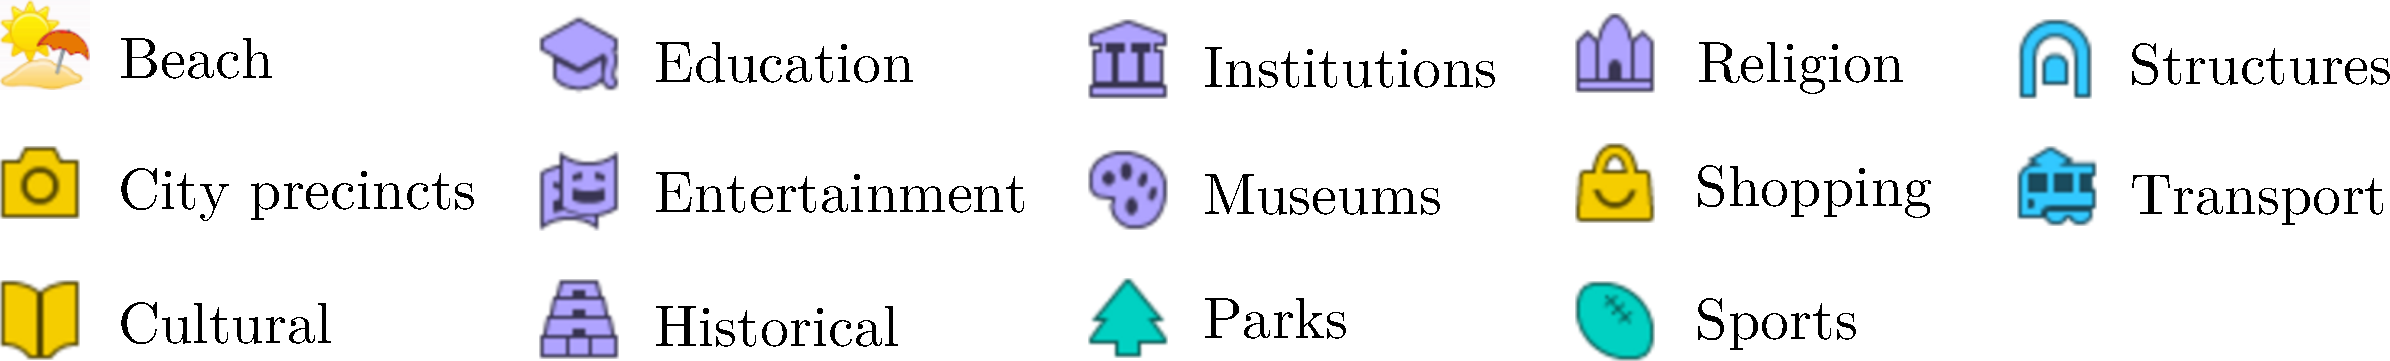
\includegraphics[width=0.7\textwidth]{fig/poi_cats_fat.pdf}
	\caption{POI Categories}
	\label{fig:poicats}
\end{figure*}


\begin{figure*}[t]
\includegraphics[width=\textwidth]{fig/feature_distro.pdf}
\caption{Distribution of POI popularity, the number of visit and visit duration}
\label{fig:distro}\captionmoveup
\end{figure*}



We described an algorithm to recommend trajectories based on ranking POIs (\textsc{PoiRank}) in Section~\ref{sec:rankplan},
the features used to rank POIs are POI and query specific, as described in Table~\ref{tab:featurerank}.

Categories of POIs in all of the five trajectory datasets are show in Figure~\ref{fig:poicats}.
The distribution of POI popularity, the number of visit and average visit duration are shown in Figure~\ref{fig:distro}.

To rank POIs, features described in Table~\ref{tab:featurerank} are scaled to range $[-1.0, 1.0]$ using the same approach 
as that utilised by libsvm (\url{http://www.csie.ntu.edu.tw/~cjlin/libsvm/}),
i.e., fitting a linear function $f(x) = a x + b$ for feature $x$ such that the maximum value of $x$ maps to $1.0$ 
and the minimum value of $x$ maps to $-1.0$.



\section{Transition Probabilities}

\begin{table}[ht]
\caption{POI features used to factorise POI-POI transition probabilities}
\label{tab:featuretran}
\centering
\setlength{\tabcolsep}{28pt} % tweak the space between columns
\begin{tabular}{l|l} \hline
\textbf{Feature}       & \textbf{Description} \\ \hline
\texttt{category}      & category of POI \\
\texttt{neighbourhood} & the cluster that a POI resides in \\
\texttt{popularity}    & (discretised) popularity of POI \\
\texttt{nVisit}        & (discretised) total number of visit at POI \\
\texttt{avgDuration}   & (discretised) average duration at POI \\ \hline
\end{tabular}
\end{table}


\begin{figure*}[b]
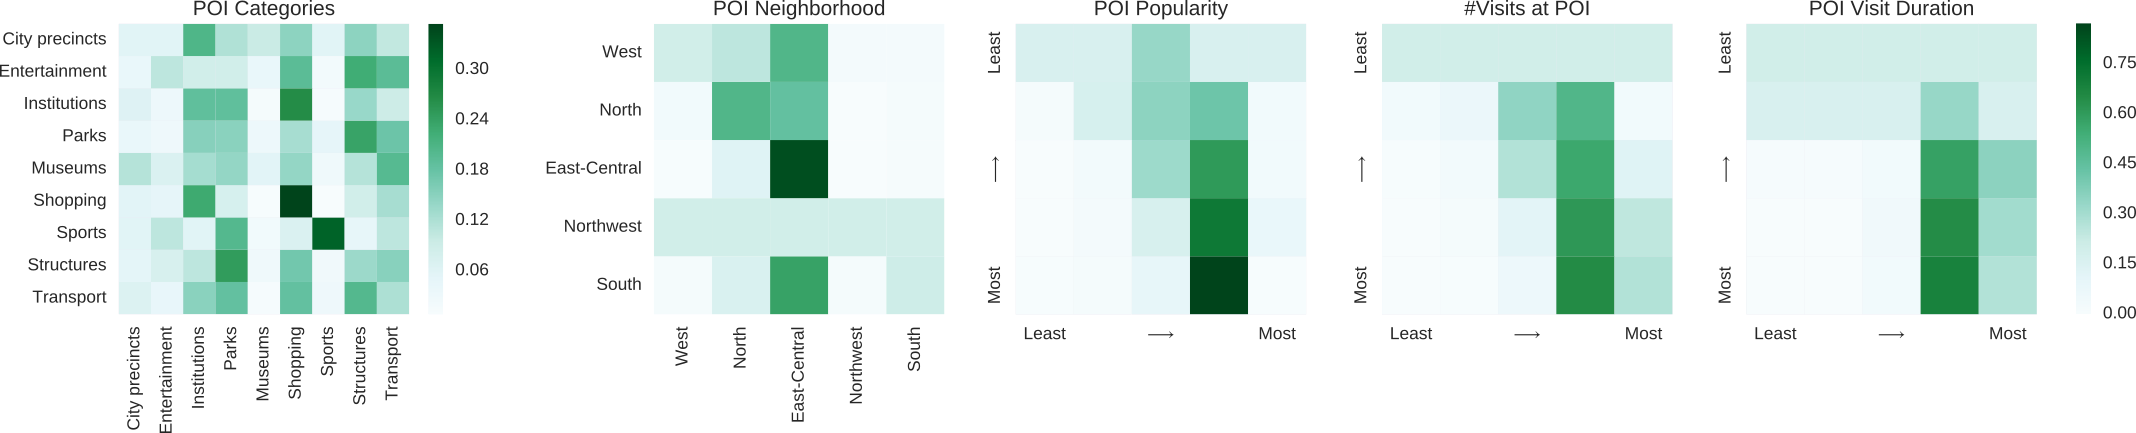
\includegraphics[width=\textwidth]{fig/poi_transmat_all.png}
\caption{Transition matrices for five POI features: POI categories, neighborhood, popularity, number of visits, and visit duration. These statistics are from the Melbourne dataset.}
\label{fig:transmat_all}
\end{figure*}

We compute the POI-POI transition matrix by factorising transition probabilities from POI $p_i$ to POI $p_j$ as a product of transition probabilities
between pairs of individual POI features, these features are described in Table~\ref{tab:featuretran}.

Transition matrices of individual POI features are computed using maximum likelihood estimation,
i.e., counting the number of transitions for each pair of features then normalising each row,
taking care of zeros by adding a small number $\epsilon$
\footnote{In our experiments, $\epsilon = 1$.}
to each count before normalisation.
Figure~\ref{fig:transmat_all} visualises the transition matrices for individual POI features in Melbourne.

The POI-POI transition matrix is computed by taking the Kronecker product of the transition matrices for the individual features,
and then updating it with two additional constraints.

Firstly, we disallow self transitions by setting probability of ($p_i$ to $p_i$) to zero.

Secondly, when a group of POIs have identical (discretised) features (say a group with $N_g$ POIs), 
we distribute the probability uniformly among POIs in the group,
in particular, the incoming (unnormalised) transition probability (say, $P_i$) of the group computed by taking the Kronecker product is divided uniformly 
among POIs in the group (i.e., $\frac{P_i}{N_g}$), which is equivalent to choose a POI in the group uniformly at random.
Moreover, the outgoing (unnormalised) transition probability of each POI is the same as that of the group, 
since in this case, \textit{the transition from any POI in the group to one outside the group represents an outgoing transition from that group}.
In addition, the self-loop transition of the group represents transitions from a POI in the group to other POIs ($N_g-1$ POIs) in the same group, 
\textit{similar to the outgoing case}, the (unnormalised) self-loop transition probability (say $P_o$) is divided uniformly (i.e., $\frac{P_o}{N_g-1}$),
which corresponds to choose a transition (from $p_i$) among all transitions to the other $N_g-1$ POIs (exclude self-loop $p_i$ to $p_i$)
in that group uniformly at random.

Lastly, we normalise each row of the (unnormalised) POI-POI transition matrix to form a valid probability distribution for each POI.



\section{Experiment}

\subsection{Dataset}
Trajectories used in experiment are extracted using geo-tagged photos in the Yahoo! Flickr Creative Commons 100M
(a.k.a. YFCC100M) dataset~\cite{thomee2016yfcc100m} as well as the Wikipedia web-pages of points-of-interests (POIs).
Photos are mapped to POIs according to their distances calculated using the Haversine formula~\cite{haversine},
the time a user arrived a POI is approximated by the time the first photo taken by the user at that POI,
similarly, the time a user left a POI is approximated by the time the last photo taken
by the user at that POI.
Furthermore, sequence of POI visits by a specific user are divided into several pieces according to
the time gap between consecutive POI visits, and the POI visits in each piece are connected in temporal order
to form a trajectory~\cite{ht10, ijcai15}.

\subsection{Parameters}
For parameters of algorithms in experiment,
we use a $0.5$ trade-off parameter for \textsc{PersTour} and \textsc{PersTour-L}, found to be the best weighting by \textsc{PersTour}~\cite{ijcai15}.
The regularisation parameter $C$ in rankSVM is $10.0$.
The trade-off parameter $\alpha$ in \textsc{Rank+Markov} and \textsc{Rank+MarkovPath} is tuned using cross validation.
In particular, we split trajectories with more than $2$ POIs in a dataset into two (roughly) equal parts, 
and use the first part (i.e., validation set) to tune $\alpha$ (i.e., searching value of $\alpha$ such that \textsc{Rank+Markov} achieves the best performance on validation set, in terms of the mean of pairs-F$_1$ scores got by leave-one-out cross validation),
then test on the second part (leave-one-out cross validation) using the tuned $\alpha$, and vice verse. 

\subsection{Implementation}
We employ the rankSVM implementation in libsvmtools (\url{https://www.csie.ntu.edu.tw/~cjlin/libsvmtools/}).
Integer linear programming (ILP) are solved using Gurobi Optimizer (\url{http://www.gurobi.com/})
and lp\_solve (\url{http://lpsolve.sourceforge.net/}).
Dataset and code for this work are available in repository \url{https://bitbucket.org/d-chen/tour-cikm16}.

\subsection{Performance metric}
A commonly used metric for POI recommendation and evaluating trajectories is
the F$_1$ score on points.
Let $\mathcal{T}$ be the trajectory that was visited in the real world,
and $\hat{\cal T}$ be the recommended trajectory,
$\mathcal{P}_{\mathcal{T}}$ be the set of POIs visited in $\mathcal{T}$,
and $\mathcal{P}_{\hat{\mathcal{T}}}$ be the set of POIs visited in $\hat{\mathcal{T}}$,
we compute F$_1$ score on points as the harmonic mean between the point-wise precision and recall,
%was defined as
\begin{displaymath}
F_1= \frac{2  P_{\textsc{point}}  R_{\textsc{point}}}
          {P_{\textsc{point}} + R_{\textsc{point}}}
\end{displaymath}
where
\vspace{-1.1em}
\begin{displaymath}%\eqmoveup
P_{\textsc{point}} = \frac{|\mathcal{P}_{\mathcal{T}} \cap \mathcal{P}_{\hat{\mathcal{T}}}|}
                          {|\hat{\mathcal{T}}|},
R_{\textsc{point}} = \frac{|\mathcal{P}_{\mathcal{T}} \cap \mathcal{P}_{\hat{\mathcal{T}}}|}
                          {|\mathcal{T}|}
\end{displaymath}

A perfect F$_1$ (i.e., F$_1 = 1$) means the POIs in
the recommended trajectory are exactly the same POIs as those in the ground truth,
and F$_1 = 0$ means that none of the POIs in the
real trajectory was recommended.

While F$_1$ score on points is good at measuring whether POIs are correctly recommended,
it ignores the visiting order between POIs.
$\text{pairs-F}_1$ takes into account both the point identity and the visiting orders in a trajectory.
This is done by measuring the F$_1$ score of every pair of ordered POIs, whether they are adjacent or not,
\begin{displaymath}
\text{pairs-F}_1 = \frac{2 P_{\textsc{pair}} R_{\textsc{pair}}}
                        {P_{\textsc{pair}} + R_{\textsc{pair}}},
\end{displaymath}
where
\vspace{-2.0em}
\begin{displaymath}%\eqmoveup
~~
P_{\textsc{pair}} = \frac{N_c} {|\hat{\mathcal{T}}|(|\hat{\mathcal{T}}|-1) / 2}, ~~
R_{\textsc{pair}} = \frac{N_c} {|\mathcal{T}|(|\mathcal{T}|-1) / 2},
\end{displaymath}
and $N_c$
\footnote{We define pairs-F$_1 = 0$ when $N_c = 0$.}
is the number of ordered POI pairs $(p_j, p_k)$ that
appear in both the ground-truth and the recommended trajectories,
\begin{align*}
    (p_j \prec_{\mathcal{T}} p_k ~\land~ p_j \prec_{\hat{\mathcal{T}}} p_k)  ~\lor~
    (p_j \succ_{\mathcal{T}} p_k ~\land~ p_j \succ_{\hat{\mathcal{T}}} p_k),
\end{align*}
with $p_j \ne p_k, ~p_j, p_k \in \mathcal{P}_{\mathcal{T}} \cap \mathcal{P}_{\hat{\mathcal{T}}}, ~1 \le j \ne k \le |\mathcal{T}|$.
Here $p_j \prec_{\mathcal{T}} p_k$ denotes POI $p_j$ was visited before POI $p_k$ in trajectory $\mathcal{T}$
and $p_j \succ_{\mathcal{T}} p_k$ denotes $p_j$ was visited after $p_k$ in $\mathcal{T}$.

Pairs-F$_1$ takes values between 0 and 1. A perfect pairs-F$_1$ (1.0) is achieved if and only if
both the POIs and their visiting orders in the recommended trajectory are exactly the same as those in the ground truth.
Pairs-F$_1 = 0$ means none of the recommended POI pairs was actually visited in the real trajectory.

Performance data reported in Table~\ref{tab:f1} and Table~\ref{tab:pairf1} are the mean and standard deviation of instances successfully recommended by
all methods shown in Table~\ref{tab:algsummary}.




\eat{
%\cheng{Report the proportion of recommended trajectories and actual trajectories with sub-tours, in the Appendix.}


\section{Markov}

\begin{algorithm}[t]
\caption{\textsc{Markov}: recommend trajectory with POI transitions}
%recommend trajectory by maximising likelihood}
\label{alg:markov}
\begin{algorithmic}[1]
\STATE \textbf{Input}: $\mathcal{P}, p_s, p_e, L$
\STATE \textbf{Output}: Trajectory $\mathcal{T} = (p_s, \cdots, p_e)$ with $L$ POIs
%\STATE Compute POI-POI transition matrix
\STATE Initialise score matrix $A$ and backtracking pointer $B$
\FOR{$p \in \mathcal{P}$}
    \STATE $A[2, p] = \log P(p|p_s)$
    \STATE $B[2, p] = p_s$
\ENDFOR
\FOR{$l=2$ to $L-1$}
    \FOR{$p \in \mathcal{P}$}
        \STATE \(\displaystyle A[l+1, p] = \max_{p' \in \mathcal{P}} \{ A[l, p'] + \log P(p|p') \} \)
        \STATE \(\displaystyle B[l+1, p] = \argmax_{p' \in \mathcal{P}} \{ A[l, p'] + \log P(p|p') \} \)
    \ENDFOR
\ENDFOR
% //trace back to find the actual path
\STATE $\mathcal{T} = \{p_e\}$, $l = L$, $p = \mathcal{T}.first$
\REPEAT
    \STATE Prepend $B[l, p]$ to $\mathcal{T}$
    \STATE $l = l - 1$, $p = \mathcal{T}.first$
\UNTIL{$l < 2$}
\RETURN $\mathcal{T}$
\end{algorithmic}
\end{algorithm}





\section{Avoid Peeking}
When working with machine learning algorithms, to make sure the reported performance is a good approximation
of the generalisation performance, it is critical to prevent information in test set from leaking into
training set.
Many algorithms shown in Table~\ref{tab:algsummary} leveraging both learning to rank and 
factorised POI-POI transition matrix,
e.g., \textsc{Rank+Markov}, \textsc{Rank+MarkovPath} and \textsc{StructuredSVM},
both of them need to be trained or parameters be estimated before being utilised in other algorithms.
POI features such as popularity, the number of visits and average visit duration are
determined by not only the POI itself but also trajectories in training set, 
let's call them aggregated features, as they are computed by aggregating a set of trajectories.
To make sure the prediction performance is reliable, 
it is very important to exclude trajectories in test set when computing aggregated features.
Unfortunately, it is quite easy, especially when utilising multiple levels of machine learning models,
to use all data, including those in test set, to compute aggregated features, 
and many researchers and practitioners did not realise the fact that 
some bits of information in test set were leaked into training set via these aggregated features.

%One may argue that many of these features will not change much when computed with or without data in test set,
%but in certain areas, such as aerodynamics, some decisions are very sensitive to the quantity of certain features.
%Nevertheless, the exact impact still needs further investigation.





\section{RankSVM}
\label{appendix:ranksvm}

\subsection{Prediction}
Given a set of $M$ POIs $\mathcal{P} = \{p_1, \cdots, p_M\}$, 
and $N$ queries $\mathcal{Q} = \{q_1, \cdots, q_N\}$.
The ranking score for POI $p_m$ with respect to query $q_n$ is 
$S_{m,n} = \langle \mathbf{w_r}, \mathbf{\phi}(p_m, q_n) \rangle$,
where $\mathbf{w_r}$ is a vector of parameters,
and $\mathbf{\phi}(p_m, q_n)$ is the scaled feature vector for $p_m$ with respect to query $q_n$,
as described in Table~\ref{tab:featurerank}.

\subsection{Training}
To estimate the parameters $\mathbf{w_r}$, we train a rankSVM with linear kernel and L$2$ loss:
%\begin{displaymath}
\begin{multline}
\min_{\mathbf{w_r}} \frac{1}{2} \mathbf{w_r}^T \mathbf{w_r} + \\ \hfill
                    C_r \sum_{(p_i, q_n), (p_j, q_n) \in \mathcal{P} \times \mathcal{Q}}
                    \max \left( 0, 1 - \mathbf{w_r}^T (\mathbf{\phi}(p_i, q_n) - \mathbf{\phi}(p_j, q_n)) \right)^2
\end{multline}
%\end{displaymath}
where $C_r > 0$ is the regularisation parameter.

The label of a training example is the number of occurrences of POI $p_m$ in trajectories grouped by query $q = (p_s, p_e, L)$,
without counting the occurrence of $p_m$ when it is the origin or destination of a trajectory.


\subsection{Structured SVM}
\label{sec:ssvm}
\secmoveup

As trajectory is a sequence of POI visits,
it is natural to model the recommended trajectory $\mathcal{T}$ with respect to query $q = (p_s, p_e, L)$
as a chain of $L$ variables, where each discrete variable has $|\mathcal{P}|$ states.
Structured prediction incorporates both the features of variables (unary features) and
the features of interactions between neighbouring variables (pairwise features) to make a
prediction,
\begin{displaymath}
    \mathcal{T}^* = \argmax_{\mathcal{T} \in \mathcal{P}^L} 
                    \sum_{j=1}^L \mathbf{w_u}^T \mathbf{\phi}_j \left( q, \mathcal{T}_j \right) +
                    \sum_{j=1}^{L-1} \mathbf{w_p}^T \mathbf{\phi}_{j, j+1} \left( q, \mathcal{T}_j, \mathcal{T}_{j+1} \right)
\end{displaymath}
where $\mathbf{\phi}_j$ are the unary features of the $j$-th variable and $\mathbf{\phi}_{j, j+1}$ are the pairwise features between
the $j$-th and $(j+1)$-th variables, $\mathbf{w_u}$ and $\mathbf{w_p}$ are the
parameters of unary and pairwise features respectively.

The unary and pairwise features are constructed from the POI ranking and POI-POI transitions.
In particular, unary features are defined as ranking probabilities (Equation~\ref{eq:poi-probability}).
Recall that we have a query consisting of start ($p_s$) and end ($p_e$) locations, which
we model as a 1-of-$K$ encoding in the unary features.
The pairwise features are defined from the transition probabilities $P(p_j | p_i)$ described in
Section~\ref{sec:transition}.
This method is called \textsc{StructuredSVM} in the experiments.

% describe SSVM training (1-slack formulation)
To estimate the parameters $\mathbf{w_u}$ and $\mathbf{w_p}$, we train a Structured Support Vector Machine
using the 1-slack formulation~\cite{ssvm09},
\begin{align*}
    \min_{\mathbf{w}, \xi \ge 0} ~~& \frac{1}{2} \mathbf{w}^T \mathbf{w} + C \xi \\
    s.t. ~~& \forall \left( \hat{\mathcal{T}}^{(1)}, \cdots, \hat{\mathcal{T}}^{(N)} \right) \in \mathscr{T}^N: \\
         ~~& \frac{1}{N} \mathbf{w}^T \sum_{i=1}^N \delta \left( \hat{\mathcal{T}}^{(i)} \right) \ge
             \frac{1}{N} \sum_{i=1}^N \Delta \left( \mathcal{T}^{(i)}, \hat{\mathcal{T}}^{(i)} \right) - \xi \\
%         ~~& \forall \hat{\mathcal{T}}^{(i)} \in \mathcal{P}^{|\mathcal{T}^{(i)}|}, i = 1, \cdots, N
\end{align*}
where $\mathbf{w} = [\mathbf{w_u}^T, \mathbf{w_p}^T]^T$ is the parameter vector,
$\mathcal{T}^{(i)}$ and $\hat{\mathcal{T}}^{(i)}$ are the $i$-th trajectory in training set
and its corresponding recommendation respectively.
$N$ is the training set size, $C$ is the regularisation parameter,
$\xi$ is the slack variable, and
\begin{displaymath}
    \delta \left( \hat{\mathcal{T}}^{(i)} \right) = \Psi \left( q^{(i)}, \mathcal{T}^{(i)} \right) - 
                                                    \Psi \left( q^{(i)}, \hat{\mathcal{T}}^{(i)} \right)
\end{displaymath}
where $q^{(i)}$ the query corresponds to the $i$-th trajectory in training set,
$\Psi \left( q^{(i)}, \mathcal{T}^{(i)} \right)$ is the joint feature vector which is a composite of unary and 
pairwise features of the $i$-th trajectory,
$\Delta \left( \mathcal{T}^{(i)}, \hat{\mathcal{T}}^{(i)} \right)$ is the loss associated with the $i$-th trajectory 
and its corresponding recommendation, and Hamming loss is used in this work.



\section{Structured SVM}
\label{appendix:ssvm}

To recommend a trajectory that starts from POI $p_s$, ends at POI $p_e$, and with $L$ POIs in total.
We build a chain with $L$ random variables (nodes) and $L-1$ directed edges between neighbouring variables,
each discrete variable has $|\mathcal{P}|$ states.
Both the first variable and the last variable are observed, i.e., they are $p_s$ and $p_e$ respectively,
all intermediate variables corresponds to POIs that should be recommended.


\subsection{Node Features}
\label{appendix:node}
Given a POI $p_m$ and a query $q_n$, the node features are the same as that described in Table~\ref{tab:featurerank}.
Features are scaled the same way as that described in Section~\ref{appendix:ranksvm}.


\subsection{Edge Features}
\label{appendix:edge}
Given an ordered pair of POIs $(p_i, p_j)$, 
the edge/pairwise features are built from the factorised transition probabilities 
according to features described in Table~\ref{tab:featuretran}:
\begin{enumerate}
\item The transition probability from the category of $p_i$ to the category of $p_j$.
\item The transition probability from the cluster with $p_i$ to the cluster with $p_j$.
\item The transition probability from the interval with the popularity of $p_i$ to the interval 
      with the popularity of $p_j$.
\item The transition probability from the interval with the number of visit at $p_i$ to the interval 
      with the number of visit at $p_j$.
\item The transition probability from the interval with the average duration at $p_i$ to the interval 
      with the average duration at $p_j$.
\end{enumerate}


\subsection{Prediction}
Given parameters for node and edge features $\mathbf{w_u}$ and $\mathbf{w_p}$, 
we can compute the score of $\mathcal{T}$ as follows:
\begin{displaymath}
S'(\mathcal{T}) = \sum_{j=1}^L     \langle \mathbf{w_u}, \mathbf{\phi}_j (\mathcal{T}_j, q) \rangle +
                  \sum_{j=1}^{L-1} \langle \mathbf{w_p}, \mathbf{\phi}_{j, j+1} (\mathcal{T}_j, \mathcal{T}_{j+1}) \rangle
\end{displaymath}
where $L = |\mathcal{T}|$ is the length of $\mathcal{T}$, 
$\mathbf{\phi}_j$ is the feature vector of the $j$-th node (variable) described in Section~\ref{appendix:node},
$q$ is the query corresponding to $\mathcal{T}$, i.e., $q = (\mathcal{T}_0, \mathcal{T}_L, L)$,
and $\mathbf{\phi}_{j, j+1}$ is the feature vector of the $j$-th edge, as described in Section~\ref{appendix:edge}.

One approach to recommend a trajectory with respect to query $q = (p_s, p_e, L)$ and parameters 
$\mathbf{w_u}$ and $\mathbf{w_p}$ is recommending the one with the maximum score, i.e.,
\begin{displaymath}
    \mathcal{T}^* = \argmax_{\mathcal{T} \in \mathcal{P}^L} S'(\mathcal{T})
\end{displaymath}


\subsection{Training}
To estimate the parameters $\mathbf{w_u}$ and $\mathbf{w_p}$, we train a Structured Support Vector Machine
using the 1-slack formulation,
\begin{align*}
    \min_{\mathbf{w}, \xi \ge 0} ~~& \frac{1}{2} \mathbf{w}^T \mathbf{w} + C \xi \\
    s.t. ~~& \forall \left( \bar{\mathcal{T}}^{(1)}, \cdots, \bar{\mathcal{T}}^{(N)} \right) \in \mathscr{T}^N: \\
         ~~& \frac{1}{N} \mathbf{w}^T \sum_{i=1}^N \delta \left( \bar{\mathcal{T}}^{(i)} \right) \ge
             \frac{1}{N} \sum_{i=1}^N \Delta \left( \mathcal{T}^{(i)}, \bar{\mathcal{T}}^{(i)} \right) - \xi
\end{align*}
where $\mathbf{w} = [\mathbf{w_u}^T, \mathbf{w_p}^T]^T$ is the parameter vector,
$C > 0$ is the regularisation parameter, $\xi$ is the slack variable, 
$N$ is the number of trajectories in training set, 
$\mathcal{T}^{(i)}$ is the $i$-th trajectory in training set, 
and its corresponding recommendation is $\bar{\mathcal{T}}^{(i)}$, and
\begin{displaymath}
    \delta \left( \bar{\mathcal{T}}^{(i)} \right) = \Psi \left( \mathcal{T}^{(i)}, q^{(i)} \right) - 
                                                    \Psi \left( \bar{\mathcal{T}}^{(i)}, q^{(i)} \right)
\end{displaymath}
where $q^{(i)}$ is the query corresponding to $\mathcal{T}^{(i)}$ and the joint feature vector of $\mathcal{T}^{(i)}$ is
\begin{displaymath}
\Psi \left( \mathcal{T}^{(i)}, q^{(i)} \right) = \left[
\left( \sum_{j=1}^{|\mathcal{T}^{(i)}|}   \mathbf{\phi}_{j}      \left( \mathcal{T}_{j}^{(i)}, q^{(i)} \right) \right)^T,
\left( \sum_{j=1}^{|\mathcal{T}^{(i)}|-1} \mathbf{\phi}_{j, j+1} \left( \mathcal{T}_{j}^{(i)}, \mathcal{T}_{j+1}^{(i)} \right) \right)^T 
\right]^T
\end{displaymath}
$\Delta \left( \mathcal{T}^{(i)}, \bar{\mathcal{T}}^{(i)} \right)$ is the loss associated with the $i$-th trajectory 
and its corresponding recommendation, and Hamming loss is used in our experiment.
}


\end{document}
